\documentclass[xcolor=table,ignorenonframetext,12pt]{beamer}
%\documentclass[xcolor=table,handout,12pt]{beamer}
\usepackage[frenchb]{babel}
\usepackage[utf8]{inputenc}
\usepackage{amsmath,amssymb}
\usepackage{graphicx}
\usepackage{pgfarrows,pgfnodes}
\usepackage{url}
\usepackage{textcomp}
\usepackage[vcentermath]{youngtab}
\usepackage{epstopdf}
\usepackage{hhline}
\usepackage{xmpmulti}
\usepackage{arcs}                       % Pour réaliser le logo TAXIPP
\usepackage{slashbox}                   % Pour réaliser le logo TAXIPP
\usepackage{MnSymbol}                   % Pour réaliser le logo TAXIPP
\PassOptionsToPackage{usenames,dvipsnames,svgnames}{xcolor} % Pour réaliser le logo TAXIPP
\usepackage{xcolor}                     % Pour réaliser le logo TAXIPP
\usepackage{multirow}
\usepackage{subfigure}
\usepackage{booktabs}
\usepackage{tikz}
\usepackage{bbold}
\usepackage{changepage}
\mode<article> {
  \usepackage{fullpage}
  \usepackage{pgf}
  \usepackage{hyperref}
}
\usepackage{tikz}
\usetikzlibrary{shapes.geometric, arrows}
\mode<presentation>
%\usetheme{Madrid}
%\usetheme[left]{Goettingen}
%\setbeamertemplate{background canvas}{\includegraphics[width=\paperwidth]{ippheader.pdf}}
\setbeamertemplate{background canvas}{\hspace{10.1cm}\includegraphics
    [width=0.2\paperwidth]{logo_ipp.pdf}}
\definecolor{ippdark}{RGB}{0,93,116}
\definecolor{ipplight}{RGB}{0,142,156}
\definecolor{ippxlight}{RGB}{0, 204, 204}
\useinnertheme[shadow=true]{rounded}
\setbeamertemplate{items}[circle]
\setbeamercolor{title}{bg=ipplight, fg=black}
\setbeamercolor{structure}{fg=ipplight}
%\setbeamertemplate{sidebar canvas left}{} % pour supprimer le fond de couleur de la barre latérale	
\setbeamertemplate{sidebar canvas left}[vertical shading][top=structure.fg!20,bottom=structure.fg!15]
\setbeamertemplate{caption}[numbered]
\setlength{\leftmargini}{12pt}
\setbeamerfont{framesubtitle}{size=\large}
\definecolor{ippdark}{RGB}{0,93,116}
\definecolor{ipplight}{RGB}{0,142,156}




% danger logo
\newcommand*{\TakeFourierOrnament}[1]{{%
\fontencoding{U}\fontfamily{futs}\selectfont\char#1}}
\newcommand*{\danger}{\TakeFourierOrnament{66}}
\newcounter{sauvegardeenumi}
\newcommand{\asuivre}{\setcounter{sauvegardeenumi}{\theenumi}}
\newcommand{\suite}{\setcounter{enumi}{\thesauvegardeenumi}}
\newenvironment{checklist}[1]{\begin{list}{$\surd$}{}#1}{\end{list}}%


\newlength{\offsetpage}
\setlength{\offsetpage}{1.0cm}
\newenvironment{widepage}{\begin{adjustwidth}{-\offsetpage}{-\offsetpage}%
		\addtolength{\textwidth}{2\offsetpage}}%
	{\end{adjustwidth}}


% Macro d'inclusion de graphiques pdf %
\newcommand{\graphique}[2][1]{\begin{minipage}{\linewidth}\begin{center}\includegraphics[width=#1\linewidth,clip]{Graphiques/#2}\end{center}\end{minipage}}

\newcommand{\os}[2]{\onslide+<#1->{#2}}%

\newcommand{\m}[2]{\multicolumn{#1}{c}{#2}}%
\newcommand{\ml}[2]{\multicolumn{#1}{l}{#2}}%
\newcommand{\tth}{\textsuperscript{th}}%
\newcommand{\nde}{\textsuperscript{nde}}
\newcommand{\er}{\textsuperscript{er}}
\newcommand{\eme}{\textsuperscript{ème}~}
\newcommand{\hligne}{\begin{tikzpicture}[remember picture,overlay]\node[shift={(-10.5 cm,-1.2cm)}]at(current page.north east){\begin{tikzpicture}{\draw[line width=0.2mm,color=ipplight,overlay](0,0)--(8,0);}\end{tikzpicture}};\end{tikzpicture}\vspace{-0.8cm}}
\newcommand{\hlignee}{\begin{tikzpicture}[remember picture,overlay]\node[shift={(-10.5 cm,-1.2cm)}]at(current page.north east){\begin{tikzpicture}{\draw[line width=0.2mm,color=ipplight,overlay](0,0)--(8,0);}\end{tikzpicture}};\end{tikzpicture}}

% MTABLE: macro for tables %
\newenvironment{mfigure}[4][1]{\def\TMP{#3}\newdimen\TMPsize\settowidth{\TMPsize}{\TMP}
\begin{figure}\caption{#2}\begin{center}\begin{tiny}
\begin{minipage}{#1\textwidth}\resizebox{\textwidth}{!}{#3}\end{minipage}
\if!#4!\empty \else \\
\resizebox{#1\textwidth}{!}{\begin{minipage}{\TMPsize}\begin{tiny}\smallskip\par
#4 \end{tiny}\end{minipage}} \fi}
{\end{tiny}\end{center}\end{figure}}

% Macro pour créer un tableau (avec notes optionnelles) %
\newenvironment{tab}[4][1]
{\def\TMP{#3}\newdimen\TMPsize\settowidth{\TMPsize}{\TMP}
\begin{table}[!ht]
\begin{center}
\begin{minipage}{14cm}
\caption{#2}
\end{minipage}
\end{center}
\begin{center}
\begin{minipage}{#1}
\resizebox{\textwidth}{!}{#3}
\end{minipage}
\if!#4!\empty \else \\
\begin{scriptsize}
\begin{minipage}{#1}\vspace{0.2cm} \par #4
\end{minipage}
\end{scriptsize} \fi }
{\end{center}
\end{table}}

\newenvironment{choixmarges}[2]{\begin{list}{}{%
\setlength{\topsep}{0pt}%
\setlength{\leftmargin}{0pt}%
\setlength{\rightmargin}{0pt}%
\setlength{\listparindent}{\parindent}%
\setlength{\itemindent}{\parindent}%
\setlength{\parsep}{0pt plus 1pt}%
\addtolength{\leftmargin}{#1}%
\addtolength{\rightmargin}{#2}%
}\item }{\end{list}}


\beamertemplatenavigationsymbolsempty


\makeatletter
\def\PENSIPP{PENS\kern-.05em\lower-.19ex\hbox{${\color{BlueGreen} \scalebox{1.4}{\underarc[1]{\overarc[1]{\textcolor{black}{\scalebox{0.7}{ipp}}}}}}\hspace{0.5ex}$}\@}
\makeatother

% numérotation de slides
\setbeamertemplate{footline}[frame number]



\title{Modeling the Careers \\ of French Public Servants: \\ A New Approach}
\author{ Mahdi Ben Jelloul*, \textbf{Lisa Degalle}* \& Simon Rabaté*}
\institute{
  \inst{*} Institut des politiques publiques
}
\subject{}

\setbeamercolor{alerted text}{fg=green}

\date{IMA 6$^{\text{th}}$ World Congress\\
	Torino, June $21^{st}$ 2017}


\AtBeginSection[]
{
	\begin{frame}[noframenumbering]
	\frametitle{\large Outline}
	\small \tableofcontents[currentsection,hideothersubsections, subsectionstyle=hide]
\end{frame}
}

\begin{document}


\frame{\maketitle}




%%%%%%%%% Section 2 -  Data %%%%%%%%%%%
\section{Data}
\begin{frame}
\frametitle{Data}

\textbf{Exhaustive administrative data}
	\begin{itemize}
	\item 2.8 m. agents born between 1940 and 1995
	\item Complete careers' record of individuals working trajectories
	\item But some key variables only available from 2011 onward:
		\begin{itemize}
		\item[$\Rightarrow$] Focus on the 2011-2015 period
		\item[$\Rightarrow$] Procedure to retrieve time spent in the rank from partial information before 2011
		\end{itemize}
	\end{itemize}
	
\vspace{0.1cm}		
\textbf{Sample selection}		
	\begin{itemize}
	\item Focus on a specific section: LTA (biggest section)
	\item Selection of individuals:
		\begin{itemize}
		\item Working in the LTA section in 2011 
		\item Work in their 2011 rank during the time they spend in it
		\item Only clean trajectories (no missing, consistent with the law) 	
		\end{itemize}
	\item[$\Rightarrow$] 97,765 workers
	\end{itemize}

\end{frame}





%%%%%%%%% Section 3 -  Graphical evidence %%%%%%%%%%%

\section{Empirical strategy}

\begin{frame}
\frametitle{Why microsimulating rank advancement}
\begin{itemize}
	\item Summary of possible career transitions
\begin{itemize}
	\item From one \textbf{level} to the next one, within a rank
%	\item[] $\Rightarrow$ Implies a strict increase in the wage index
	\item From one \textbf{rank} to the next one, within a section
%	\item[] $\Rightarrow$ Implies a weak increase in the wage index and a change of salary grid\\
	\item From one \textbf{section} to another one
%	\item[] $\Rightarrow$ Implies a weak increase in the wage index and a change of salary grid\\
\end{itemize}
	\item We could simulate changes between levels or sections. But:
	\begin{enumerate}
		\item Level advancement is deterministic, by law
		\item The vast majority of job-to-job changes happens within a section %From one year to another:
		\item Conditions for rank advancement seem to have a large impact on job rank
	\end{enumerate}
\end{itemize}
\end{frame}





\begin{frame}
\frametitle{Why microsimulating rank advancement}
	\begin{enumerate}
	\item Level advancement is deterministic
	\begin{itemize}
	\item Most agents changing level do so after having spent the minimal required time in their level
	\end{itemize}
	\vspace{-0.1cm}
	\begin{center}
		\begin{figure}
			\includegraphics[width=.75\textwidth]{Graphiques/distrib_level.pdf}
		\end{figure}
	\end{center}
	\asuivre
\end{enumerate}
\end{frame}

\begin{frame}
\frametitle{Why microsimulating rank advancement}

\begin{enumerate}
	\suite
	\item The vast majority of job-to-job change happens within a section. From one year to another:
	\begin{itemize}
		\item 98 \% of the LTA agents remain in their section
		\item 85 \% of the LTA who advance rank remain in their section
		\item Same results for the vast majority of the sections
	\end{itemize}
	\asuivre
\end{enumerate}
\end{frame}

\subsection{Global analysis of transitions}

\subsection{Evidence of the impact of institutional conditions}


\begin{frame}




\frametitle{Why microsimulating rank advancement}
\begin{enumerate}
	\suite
	\item Conditions for rank advancement seem to have a large impact on rank advancement.
\end{enumerate}
\begin{itemize}
	\item Recall the conditions for rank advancement in our sample:
\end{itemize}
\begin{table}
\small
\begin{tabular}{l|c|cc}

\toprule
 Rank  & Type &  \multicolumn{2}{c}{Conditions}  \\
		&  			&  Duration condition	&  Level condition \\
\midrule
1  &	Ex. pro. 	&   3y in rank  & 	4  \\
1  &	Eval. committee 	& 	10y in rank &	7   \\ \midrule
2  & 	Eval. committee		& 	6y in section  &	5   \\ \midrule
3  & 	Eval. committee		& 	5y in rank  &	6   \\	
%	
\bottomrule
\end{tabular}
\end{table}

\end{frame}


\begin{frame}
\frametitle{Graphical evidence for Rank 3}
\begin{itemize}
	\item Hazard rate by duration in rank
\end{itemize}
\vspace{-0.2cm}
\begin{center}
\begin{figure}
\includegraphics[width=.75\textwidth]{Graphiques/hazard_by_duree_TTH3.pdf}
\end{figure}
\end{center}
\end{frame}

\begin{frame}
\frametitle{Graphical evidence for Rank 3}
\begin{itemize}
	\item Hazard rate by level
\end{itemize}
\vspace{-0.2cm}
\begin{center}
\begin{figure}
\includegraphics[width=.75\textwidth]{Graphiques/hazard_by_ech_TTH3.pdf}
\end{figure}
\end{center}

\end{frame}
\begin{frame}
\frametitle{Graphical evidence for Rank 3}
\begin{itemize}
	\item Hazard rate by distance to the thresholds
\end{itemize}
\vspace{-0.2cm}
\begin{center}
\begin{figure}
\includegraphics[width=.75\textwidth]{Graphiques/hazard_by_dist_TTH3.pdf}
\end{figure}
\end{center}

\end{frame}


\begin{frame}
\frametitle{Logit estimation}
\framesubtitle{Model}
\begin{choixmarges}{-0.7cm}{-0.7cm}


\begin{itemize}
\item Difficulty: dealing with different type of rank change\\ (rank 1: 2 conditions, rank 2 and 3: 1 condition).
\item Simplification at this stage: consider only the first condition reached for all ranks
\item Specification:



\small
\begin{equation*}
\begin{array}{c l}
log \frac{P(Change=1)}{1 - P(Change=1)} =& \alpha  + \delta X + \beta \mathbb{1}_{{\text{conditions fullfiled}}} 
\end{array} 
\end{equation*}

With :
\vspace{-0.1cm}
\begin{equation*}
\left\{\begin{array}{c  l}
\mathbb{1}_{{\text{conditions fullfiled}}}   &= \text{dummy if rank-related conditions are fullfiled}  \\
X &= \text{gender, rank, duration in rank} \\
\end{array} \right.  
\end{equation*}
\normalsize


\item Sample: all transitions observed between 2011 and 2014.

\end{itemize}

\end{choixmarges}

\end{frame}


%%%%%%%%% Section 3 -  Duration analysis %%%%%%%%%%%
%\section{Survival analysis}


%\subsection{Censoring}
%
%
%
%\begin{frame}
%\frametitle{Censoring}
%\begin{center}
%\begin{figure}
%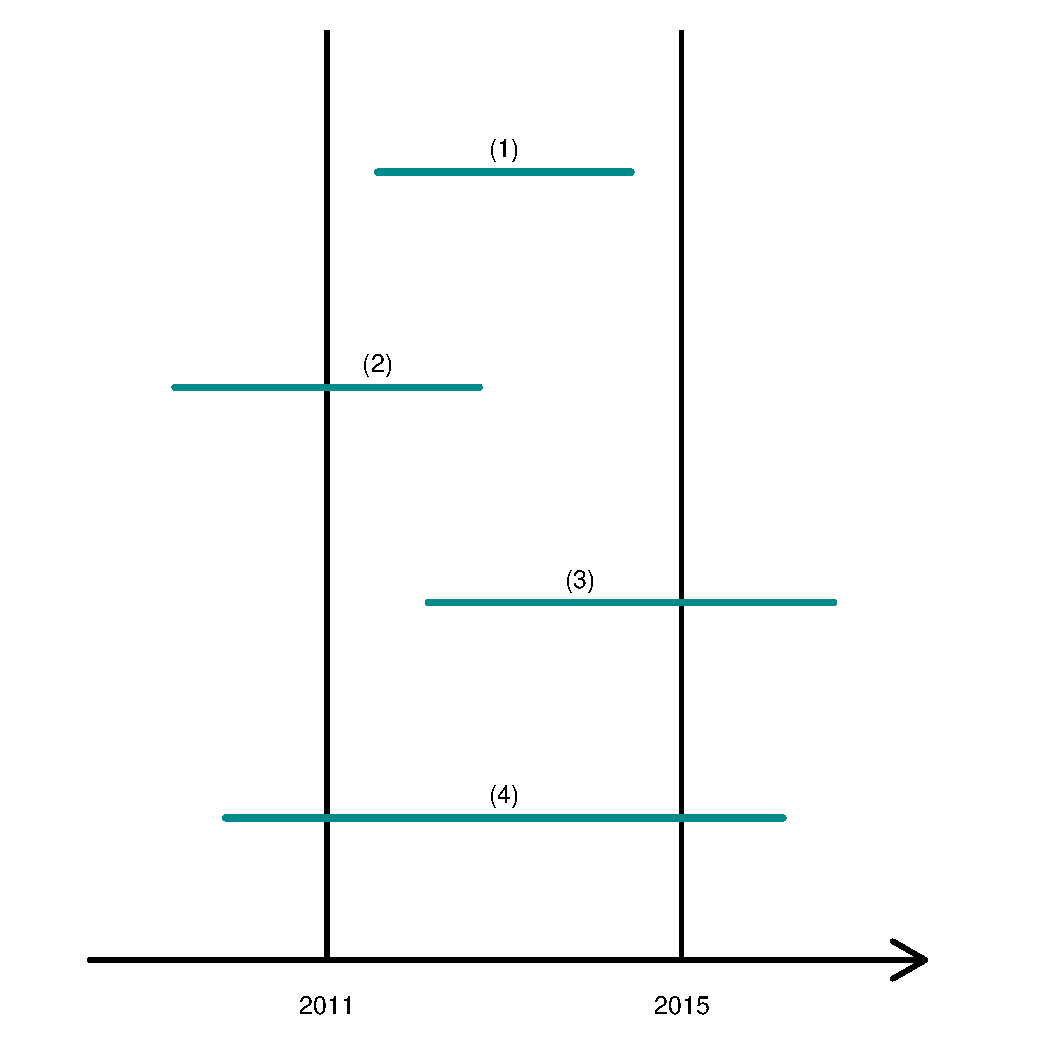
\includegraphics[width=.5\textwidth]{Graphiques/schema_censoring.pdf}
%\end{figure}
%\end{center}
%$\Rightarrow$ Uniquement les cas (2) et (4) ici car 
%
%\begin{table}[ht]
%\centering
%\begingroup\footnotesize
%\begin{tabular}{lccccc}
%  \hline
% & All & TTH1 & TTH2 & Rank 3 & TTH4 \\ 
%  \hline
%\% right-censored & 0.567 & 0.670 & 0.198 & 0.320 & 0.757 \\ 
%  \% left-censored & 0.086 & 0.112 & 0.013 & 0.021 & 0.058 \\ 
%   \hline
%\end{tabular}
%\endgroup
%\end{table}
%
%\end{frame}
%
%
%
%\begin{frame}
%\frametitle{Censoring}
%\begin{center}
%\begin{figure}
%
%
%
%
%\end{frame}
%
%
%
%
%\subsection{Estimations}


%%%%%%%%% Section 4 -  Estimation %%%%%%%%%%%
\section{Results}

\subsection{Estimation}


\begin{frame}
\frametitle{Logit estimation : \large Results}
\begin{choixmarges}{-0.5cm}{-0.5cm}
\vspace{0.1cm}
\begin{table}
\begin{center}
\scriptsize
\resizebox*{0.9\textwidth}{8.5cm}{\begin{tabular}{l c c c }
\toprule
 & Model 1 & Model 2 & Model 3 \\
\midrule
I\_threshold   & $0.102^{***}$ & $0.098^{***}$  &                \\
               & $(0.001)$     & $(0.005)$      &                \\
Rank 2         & $0.277^{***}$ & $0.274^{***}$  & $0.268^{***}$  \\
               & $(0.003)$     & $(0.003)$      & $(0.003)$      \\
Rank 3         & $0.244^{***}$ & $0.243^{***}$  & $0.166^{***}$  \\
               & $(0.003)$     & $(0.003)$      & $(0.003)$      \\
Rank 4         & $0.090^{***}$ & $0.095^{***}$  & $-0.027^{***}$ \\
               & $(0.006)$     & $(0.006)$      & $(0.003)$      \\
sexe = M       & $0.021^{***}$ & $0.021^{***}$  & $0.019^{***}$  \\
               & $(0.001)$     & $(0.001)$      & $(0.001)$      \\
duration\_bef  &               & $0.001$        &                \\
               &               & $(0.003)$      &                \\
duration\_bef2 &               & $-0.000$       &                \\
               &               & $(0.000)$      &                \\
duration\_aft  &               & $0.004^{***}$  &                \\
               &               & $(0.001)$      &                \\
duration\_aft2 &               & $-0.001^{***}$ &                \\
               &               & $(0.000)$      &                \\
duration       &               &                & $0.030^{***}$  \\
               &               &                & $(0.001)$      \\
duration2      &               &                & $-0.002^{***}$ \\
               &               &                & $(0.000)$      \\
\midrule
Num.\ obs.     & 293423        & 293423         & 293423         \\
AIC            & 200576.312    & 200510.190     & 204883.701     \\
\bottomrule
\multicolumn{4}{l}{\scriptsize{$^{***}p<0.01$, $^{**}p<0.05$, $^*p<0.1$}}
\end{tabular}}
\end{center}
\end{table}


\end{choixmarges}

\end{frame}



\subsection{Simulation}

\begin{frame}
\frametitle{Simulation}
\framesubtitle{Adequacy tests}
\begin{choixmarges}{-0.5cm}{-0.5cm}


\begin{itemize}

\item MS model: assessment of the quality of the model based on its predictability
\vspace{0.2cm}

\item Ideal test: ability of the model to predict the dynamic of rank exit between 2011 and 2014
	\begin{itemize}
	\item Requires to model the counterfactual level evolution for those exiting before 2015
	$\Rightarrow$ Not done yet
	\end{itemize}
\vspace{0.2cm}

\item Tests used so far: 2011 only
	\begin{itemize}
\item Split the main sample in two (learning/test samples)
\item Estimate the models on the learning sample 
\item Predict rank exit between 2011 and 2012 from the coefficients in the test sample
\item Compare observed vs. predicted exit
	\end{itemize}

\end{itemize}
\end{choixmarges}

\end{frame}


\begin{frame}
\frametitle{Simulation}
\framesubtitle{Results}
\begin{choixmarges}{-0.5cm}{-0.5cm}

\begin{table}[ht]
\centering
\begingroup\footnotesize
\begin{tabular}{lcccc}
  \toprule
 & Observed & Null model & Model 2 & Model 3 \\ 
  \midrule
\% exit All & 0.130 & 0.128 & 0.127 & 0.127 \\ 
\% exit rank1 & 0.072 & 0.129 & 0.074 & 0.075 \\ 
\% exit rank2 & 0.347 & 0.128 & 0.317 & 0.313 \\ 
  \% exit rank3 & 0.192 & 0.126 & 0.191 & 0.208 \\ 
  \% exit rank4 & 0.080 & 0.118 & 0.076 & 0.054 \\ 
   \midrule
     \textbf{Mean wage index }& \textbf{342} & 328 & \textbf{340} & 336 \\ 
  Q1 index & 310 & 303 & 310 & 310 \\ 
  Median index & 328 & 310 & 323 & 323 \\ 
  Q3 index & 364 & 336 & 360 & 351 \\ 
 \bottomrule 
\end{tabular}
\endgroup
\end{table}

\vspace{0.2cm}
\begin{itemize}
\item[$\Rightarrow$] Better fit for the model \textbf{with the institution constraints}

\end{itemize}


\end{choixmarges}

\end{frame}



\section{Conclusion and next steps}


\begin{frame}

\frametitle{Results}

\begin{choixmarges}{-0.5cm}{-0.5cm}
\begin{enumerate}
\vspace{0.2cm}
\item Impact important des conditions institutionnelles ...
\begin{itemize}
\item Statistiques descriptives pour visualiser l'impact des conditions, séparément et en cumulé
\item Effet important dans les estimations
\end{itemize}

\vspace{0.2cm}
\item ... Mais pas d'effets sensibles sur les simulations
\begin{itemize}
\item L'ajout des variables institutionnelles n'améliore pas le fit
\item Surprenant vue la magnitude de l'effet
\item[$\Rightarrow$] Résultat non définitif
\end{itemize}

\end{enumerate}
\end{choixmarges}
\end{frame}



\begin{frame}

\frametitle{Next steps}

\begin{choixmarges}{-0.5cm}{-0.5cm}

\begin{itemize}

\begin{itemize}

\item Modeling choice of next rank using multichoice models
\begin{itemize}
\item Choix multiples (logit multinomial, emboité?)
\item Modèles de durée
\end{itemize}

\vspace{0.1cm}

\item Améliorer la procédure de test des modèles
\begin{itemize}
\item Sur 2011-2014 (modélisation des échelons)
\item D'autres critères d'évaluations ? 
\end{itemize}

\end{itemize}

\vspace{0.2cm}


\item Questions plus générales:
\begin{itemize}
\item Généralisation des résultats aux autres corps ?
\item Mise en oeuvre dans le modèle
\item Articulation avec les autres modules (affiliation, marché du L)
\end{itemize}

\end{itemize}



\end{choixmarges}
\end{frame}



\end{document}

%\section*{Appendix: Completion of career trajectories before 2011}
%
%
%
%
%\subsection{Method}
%\begin{frame}
%\frametitle{Algorithme}
%\begin{itemize}
%\item Pour chaque année de 2011 à 2003, pour chaque agent qui n'a pas encore atteint son année d'entrée dans son rank de 2011, on suit cet arbre de décision pour identifier une année d'entrée dans le rank de 2011 :\\
%\end{itemize}
%\bigskip
%
%\tikzstyle{startstop} = [rectangle, rounded corners, minimum width=0.5cm, minimum height=0.5cm,text centered, draw=black, fill=ipplight]
%\tikzstyle{io} = [trapezium, trapezium left angle=70, trapezium right angle=110, minimum width=1cm, minimum height=1cm, text centered, draw=black, fill=ippdark]
%\tikzstyle{process} = [rectangle, minimum width=0.5cm, minimum height=0.5cm, text centered, draw=black, fill=ippxlight]
%\tikzstyle{decision} = [diamond, minimum width=0.5cm, minimum height=0.5cm, text centered, draw=black, fill=ippdark]
%\tikzstyle{arrow} = [thick,->,>=stealth]
%
%\begin{widepage}
%\begin{center}
%\resizebox{1\textwidth}{3.cm}{
%\begin{tikzpicture}[node distance=5cm, sibling distance = 7cm]
%
%\node (start) [startstop, xshift=-3cm, yshift=6cm] {$IB_{t-1}$ sur grille $Grade_{t}$?};
%\node (in1) [process, right of=start, xshift=2.5cm] {$Grade_{t}$ = TTH1?}
%	child { node {$!\Delta$, $Grade_{t-1}$ = TTH1} edge from parent node[left,draw=none] {oui}}
%	child { node (start3) [startstop] {$IB_{t-1}$ sur grille $(Grade-1)_{t}$?} 
%		child[yshift=-0.5cm] { node {\begin{tabular}{c} ambigu: \\ !$\Delta$, $Grade_{t-1}$ =  $(Grade-1)_{t}$ ou\\ $\Delta$, $Grade_{t-1}$ =  $(Grade)_{t}$ \end{tabular}} 	edge from parent node[left,draw=none] {oui}}
%		child { node {$!\Delta$, $Grade_{t-1}$ = $Grade_{t}$} 	edge from parent node[right,draw=none] {non}}
%		edge from parent node[right,draw=none] {non} }
%	;
%
%\node (in2) [process, left of=start, xshift=-1.5cm] {$Grade_{t}$ = TTH1?}
%child { node {$\Delta$, $Grade_{t-1}$ = autre} edge from parent node[left,draw=none] {oui}}
%child { node (start2) [startstop] {$IB_{t-1}$ sur grille $(Grade-1)_{t}$?} 
%	child{ node {$\Delta$, $Grade_{t-1}$ = autre} edge from parent node[left, draw=none] {non} }
%	child{ node {$\Delta$, $Grade_{t-1}$ = $(Grade-1)_{t}$} edge from parent node[right, draw=none] {oui} }
%	edge from parent node[right,draw=none] {non}}
%;
%
%
%\draw [arrow] (start.north) -- node[anchor=north] {oui} (in1.north);
%\draw [arrow] (start.north) -- node[anchor=north] {non} (in2.north);
%
%%\draw [arrow] (in1) -- node[anchor=east] {no} (in2);
%%
%%\draw [arrow] (in2) -- node[anchor=north] {yes} (in1);
%%\draw [arrow] (in2) -- node[anchor=east] {no} (in2);
%\end{tikzpicture}
%}
%
%\end{center}
%
%\end{widepage}
%\begin{flushright}
%	\hyperlink{chevauchements}{\beamerbutton{Graphique chevauchements}}
%\end{flushright}
%
%\end{frame}
%
%\begin{frame}[label = chevauchements]
%
%\frametitle{Appendice : chevauchements de grilles}
%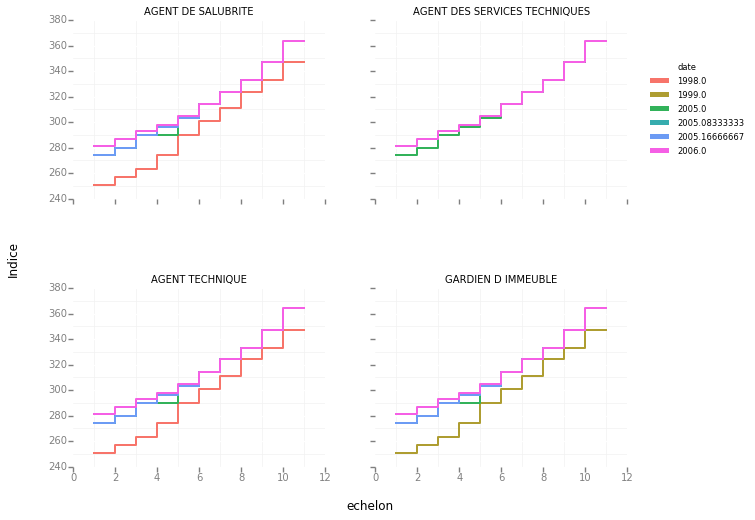
\includegraphics[width=\textwidth]{Graphiques/chevauchements.png}
%
%\end{frame}
%
%
%\subsection{Results}
%\begin{frame}
%\frametitle{Résultats}
%\begin{itemize}
%\item Différence entre l'année d'entrée prédite maximale et d'entrée prédite minimale dans le rank de 2011
%\end{itemize}
%\begin{figure}
%\vspace{-0.5cm}
%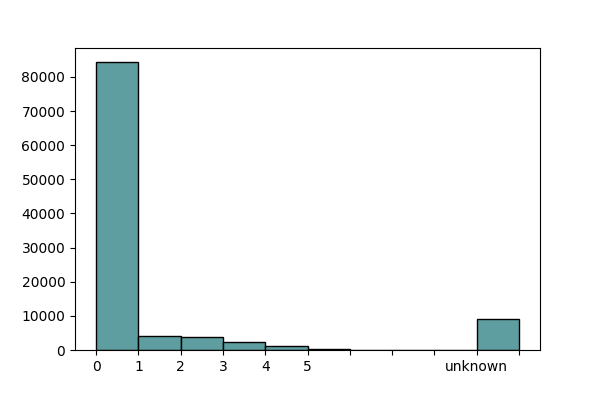
\includegraphics[scale=0.55]{Graphiques/gap.pdf}
%\end{figure}
%
%\end{frame}
%
%\begin{frame}
%\frametitle{Resultats - suite}
%\begin{itemize}
%	\item Effectifs par année d'entrée dans le rank de 2011
%\end{itemize}
%\begin{center}
%	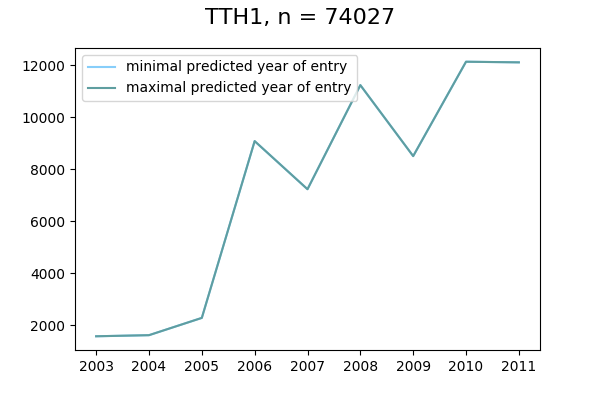
\includegraphics[width=.4\textwidth]{Graphiques/survival_TTH1.pdf}
%	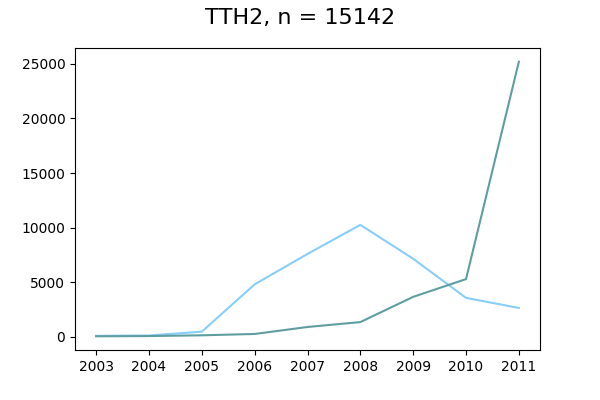
\includegraphics[width=.4\textwidth]{Graphiques/survival_TTH2.pdf}
%\end{center}
%\begin{center}
%	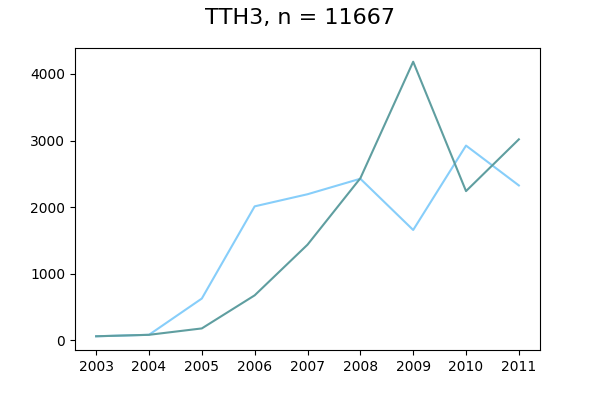
\includegraphics[width=.4\textwidth]{Graphiques/survival_TTH3.pdf}
%	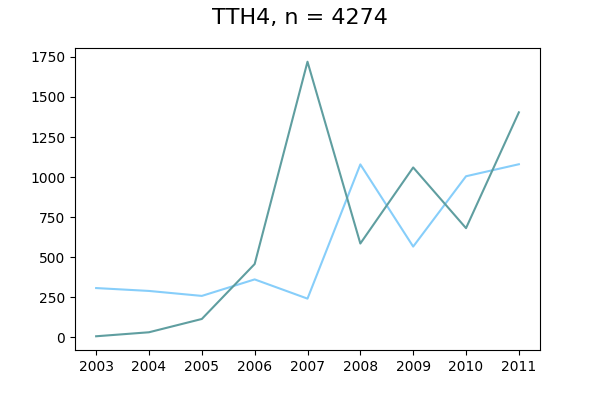
\includegraphics[width=.4\textwidth]{Graphiques/survival_TTH4.pdf}
%\end{center}
%
%\end{frame}
%
%
%\begin{frame}
%\frametitle{Resultats - suite}
%\begin{itemize}
%	\item TTH1
%\end{itemize}
%\begin{center}
%		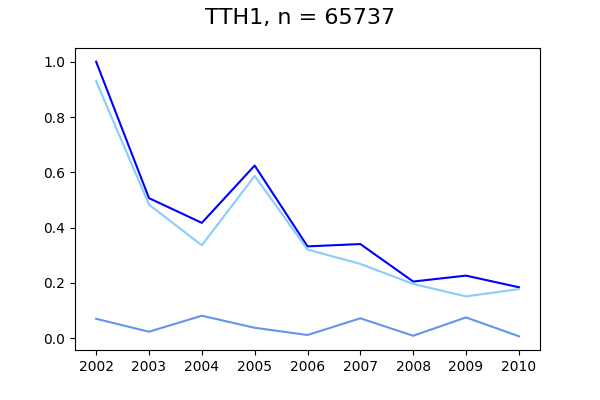
\includegraphics[width=0.55\textwidth]{Graphiques/hazards_TTH1_if_annee_min.pdf}
%\end{center}
%\begin{center}
%		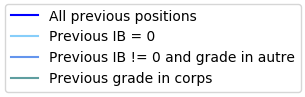
\includegraphics[width=0.3\textwidth]{Graphiques/legend.png}
%\end{center}
%\end{frame}
%
%\begin{frame}
%\frametitle{Resultats - suite}
%\begin{itemize}
%	\item TTH2
%\end{itemize}
%	\begin{center}
%	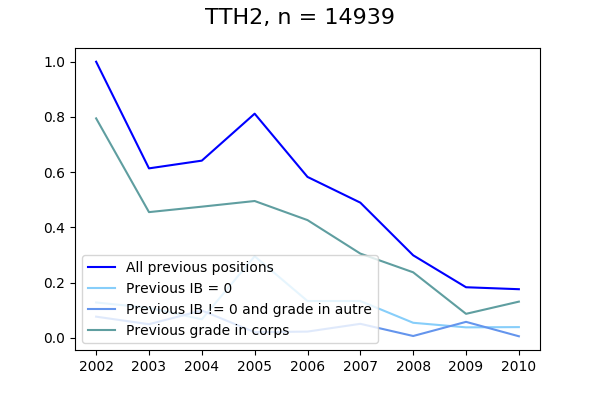
\includegraphics[width=.5\textwidth]{Graphiques/hazards_TTH2_if_annee_min.pdf}
%	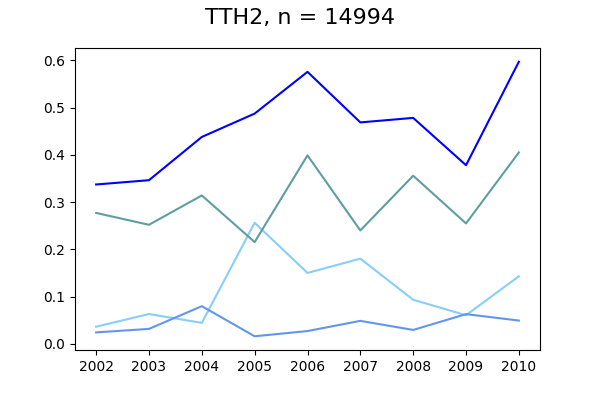
\includegraphics[width=.5\textwidth]{Graphiques/hazards_TTH2_if_annee_max.pdf}
%\end{center}
%\begin{center}
%	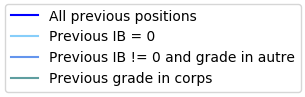
\includegraphics[width=0.3\textwidth]{Graphiques/legend.png}
%\end{center}
%
%\end{frame}
%
%
%\begin{frame}
%\frametitle{Resultats - suite}
%\begin{itemize}
%	\item Rank 3
%\end{itemize}
%\begin{center}
%	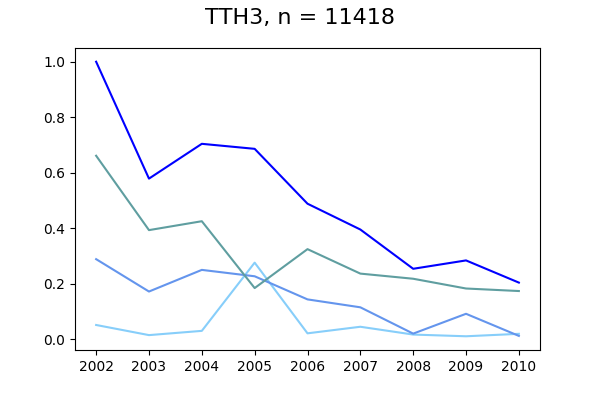
\includegraphics[width=.5\textwidth]{Graphiques/hazards_TTH3_if_annee_min.pdf}
%	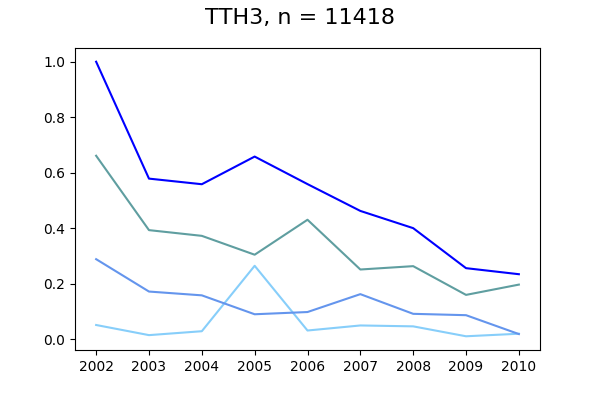
\includegraphics[width=.5\textwidth]{Graphiques/hazards_TTH3_if_annee_max.pdf}
%\end{center}
%\begin{center}
%	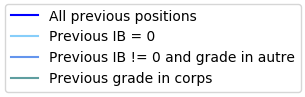
\includegraphics[width=0.3\textwidth]{Graphiques/legend.png}
%\end{center}
%
%\end{frame}
%
%\begin{frame}
%\frametitle{Resultats - suite}
%\begin{itemize}
%	\item TTH4
%\end{itemize}
%\begin{center}
%	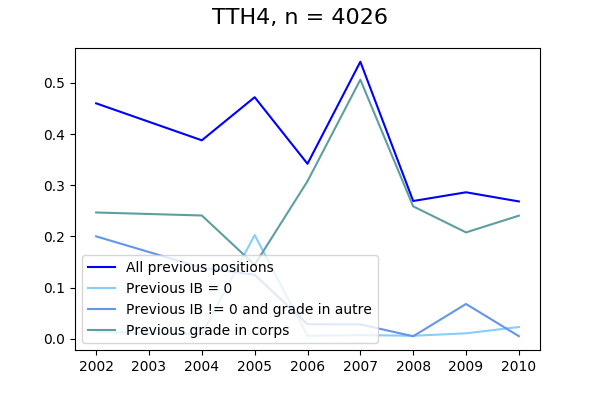
\includegraphics[width=.5\textwidth]{Graphiques/hazards_TTH4_if_annee_min.pdf}
%	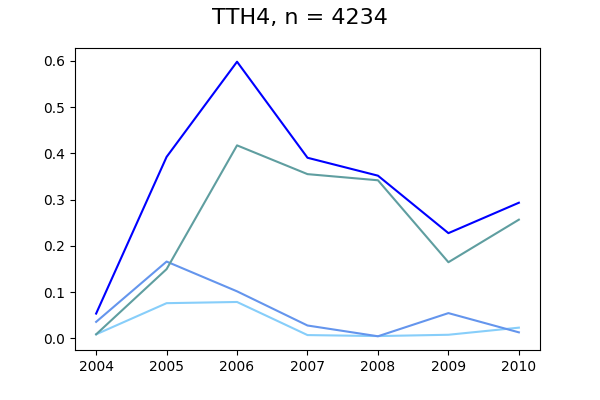
\includegraphics[width=.5\textwidth]{Graphiques/hazards_TTH4_if_annee_max.pdf}
%\end{center}
%\begin{center}
%	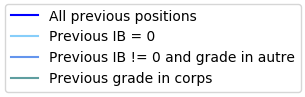
\includegraphics[width=0.3\textwidth]{Graphiques/legend.png}
%\end{center}
%
%\end{frame}
%
%
%\begin{frame}
%\frametitle{Comparaison}
%\begin{itemize}
%	\item Effectifs par année d'affiliation et par rank de 2011
%\end{itemize}
%\begin{center}
%	\includegraphics[width=.5\textwidth]{Graphiques/distrib_an_aff.pdf}
%\end{center}
%
%
%\end{frame}
%
%distrib_an_aff.pdf
%
%
%
\end{document}

% Glossaire
% dépendance: disability
